\chapter{SmartIO}\label{chapter:smartio}
SmartIO is a solution for allowing the local resources of a machine,~i.e., memory and devices, to be shared with and used by remote machines, over standard \gls{pcie}.
%
SmartIO works for \emph{all} standard \gls{pcie} devices and their Linux device drivers, no special adaptation is needed in either hardware or software to make this sharing possible.
%
Whether devices are actually local or remote becomes irrelevant to the user, as SmartIO eliminates this distinction, with regard to both functionality and performance.
%
Furthermore, individual device functions of multi-function devices may be distributed to different machines in the network, or to the same machine should it require multiple resources.
%
It is even possible to \lgls{disaggregation}{disaggregate} a single device~(function) in software, and distribute it to multiple machines, should this be required by application software.
%
In other words, SmartIO is a solution for scaling out and using more hardware resources than there are available in a single machine.


In this chapter, we provide an overview of the SmartIO solution.
%
The complete system is described in detail in \cref{paper:tocs}.
%
\Crefrange{paper:nossdav}{paper:cc} show the evolution towards this complete system, including different iterations of individual components and parts as well as gradual performance improvements.


\section{Underlying idea}\label{sec:idea}
\begin{figure}
    \centering
    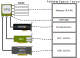
\includegraphics{bus-enumeration}
    \caption[Devices are part of the same address space as the \glsfmtshort{cpu} and system memory]
    {Device memory regions (``\acrshortpl{bar}''), are part of the same address space as \acrshort{cpu} and system memory, allowing
    the \gls{cpu} to read from and write to device memory the same way it would access \acrshort{ram}. Devices may use \gls{dma} to read from and write to \acrshort{ram}.}
    \label{fig:bus-enumeration}
\end{figure}
The defining feature of \gls{pcie} is that devices are mapped into the same address space as the \gls{cpu} and \gls{ram}, as seen in \cref{fig:bus-enumeration}.
%
This allows a \gls{cpu} to read from and write to device memory in the same manner it would access \gls{ram}.
%
Likewise, devices capable of \gls{dma} may read from and write to \gls{ram} directly.
%
\Gls{pcie} also uses \gls{msi}, allowing devices to raise interrupts by writing to an address reserved by the \gls{cpu} instead of requiring dedicated interrupt lines.



This mapping occurs when a system enumerates the \gls{pcie} bus and accesses the configuration space of each device.
%
The configuration space contains a description of the capabilities of a device, such as its memory regions.
%
The system will reserve a memory address range for each of these device memory regions.
%
By writing the start address of these regions to the device's \glspl{bar}, a device is made aware of the address space mapping.
%
As such, the term ``\gls{bar}'' is used interchangeably for a region of device memory.
%
In addition, addresses reserved by the system for interrupts are also written to the device's configuration space.



\begin{figure}
    \centering
    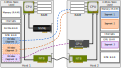
\includegraphics{ntb-example}
    \caption[Two computer systems connected using \glsfmtshortpl{ntb}, and the \glsfmtshortpl{ntb} translate between the two different address domains]
    {Two computer systems connected together using \glspl{ntb} and external cables. Host~1 has mapped segments of Host~2's memory through its local \gls{ntb}, providing Host~1 with ``windows'' into the remote system's address space. The \glspl{ntb} translate addresses between the two independent address domains.}
    \label{fig:ntb-example}
\end{figure}


As depicted in \cref{fig:ntb-example}, it is possible to connect computer systems with different address domains together over \gls{pcie} by using \glspl{ntb}.
%
\Glspl{ntb} can be embedded as a \gls{cpu} feature~\cite{whitepaper:Sullivan2010,url:LinuxNTB-AMD}, but are more commonly implemented in \gls{pcie} switch chips~\cite{whitepaper:PLX,pex8733}.
%
Using such \gls{ntb}-capable switch chips to implement peripheral devices, independent computer systems can connect with plug-in host adapter cards and external cables.
%
To the system, the \gls{ntb} appears as a normal \gls{pcie} device with one or more memory regions, or \glspl{bar}, which are reserved and mapped during the enumeration process.
%
However, rather than being backed by device registers or memory on the device, the \gls{ntb} instead forwards reads and writes to these \glspl{bar} from one side of the \gls{ntb} to the other, translating memory addresses in the process.
%
The \gls{ntb} uses a look-up table for address translation, which can be configured dynamically during run-time.
%
By using different base offsets, it is possible to configure several memory-mappings (or ``windows'') into remote memory.
%
\Cref{fig:ntb-example} illustrates how arbitrary memory addresses on the remote system can be mapped, allowing the local \gls{cpu} to access memory on a remote system as if it was local device memory.
%
Even memory on a remote \emph{device} may be mapped this way, as devices on the remote system are part of the same address space as memory~(\gls{ram}).
%
It should be noted that because the \gls{ntb} look-up table is implemented in \gls{ntb} hardware, address translation between the different domains is very fast, but the number of \gls{ntb} windows is limited by the maximum number of table entries.








%\paperref{tocs}{pcie-addr}



\section{Implementation}\label{sec:impl}

%\paperref{tocs}{pcie-addr}
\begin{itemize}
    \item a combined (and \textbf{shortened}!!) version of PCIe overview + NTB + mapping bars and DMA windows from previous papers
    \item simple ntb figure for mapping memory on remote node
    \item the famous device lending figure (but in a ``is this possible?'' kind of way)
    \item the general idea: can stuff (memory + bars + interrupts) be mapped through the NTB in a way that is transparent for OS?
\end{itemize}


%Unlike existing solutions for distributed \gls{io}, SmartIO seamlessly combines traditional \gls{io} with distributed shared-memory functionality, and is, therefore, able to provide sharing capabilities at multiple abstraction levels.
%Devices may be distributed to physical hosts and to \glspl{vm} alike, and SmartIO also provides facilities for \glslink{disaggregation}{disaggregating} devices and memory resources in software.


%However, as resources are accessed over native \gls{pcie}, they can be shared and used by remote machines without introducing a performance penalty.
%%
%Also unlike existing \gls{pcie}-based solutions, SmartIO is fully distributed and avoids dedicated servers.
%All machines in the cluster can contribute their own local resources and access remote resources, even at the same time.
%%
%Finally, by using \gls{pcie} shared memory techniques, SmartIO is able to abstract away the physical location of devices and memory resources. 
%Memory addresses are translated between different address domains by SmartIO in a manner that is transparent to application software, device drivers, and even the \gls{os}.
%This makes it possible to provide optimizations based on resource locality and minimizing data movement, without requiring the user to be aware of the underlying PCIe topology.
%\section{General idea}\label{sec:idea}
High level explanation of borrowers and lenders here.
Software architecture figure (showing the different components here)

\subsection{Device Lending}
\begin{itemize}
    \item explain shadow device
    \item intercept configuration cycles
    \item hooking DMA api for setting up DMA windows
    \item IOMMU discussion
\end{itemize}

\subsection{MDEV}
\begin{itemize}
    \item \textbf{very} brief: what is passthrough/VFIO
    \item what MDEV gives us
    \item how to map VM memory for device
    \item relaying interrupts
\end{itemize}

\subsection{API extension}
\begin{itemize}
    \item why do we need API? (disaggregation in software + shared memory networking)
    \item short explanation of SISCI
    \item what functions did we add to SISCI?
\end{itemize}

\subsection{Support for multiple lenders}
\begin{itemize}
    \item peer-to-peer device lending
    \item peer-to-peer vms
\end{itemize}


\subsection{NVMe driver}\label{sec:nvme}
\begin{itemize}
    \item why a prototype driver? demonstrate disaggregation in software
    \item why nvme? easy to parallelize because of queues
    \item driver implementation and queue sharing
    \item gpudirect + co-operation with device lending
\end{itemize}

%\section{Workload}\label{sec:eval}

\section{Performance measurements}\label{sec:eval}
Some selected performance graphs here, demonstrating zero-overhead :)

\section{Related work}\label{sec:rw}
should rw go in discussion and conclusion instead?
\begin{itemize}
    \item rdma stuff
    \item fabric partitioning: mr-iov, broadcom/microsemi chips with partitioning
    \item ladon (and other ntb stuff)
    \item disaggregation
\end{itemize}

% RW first??
%An example of this is rCUDA, where multiple clients may run jobs on the same \gls{gpu} by relying ~\cite{Duato2010}
%\Gls{rdma}-based \gls{disaggregation} can even allow a single resource to be shared by several machines in the cluster at the same time. 
%
%However, since 
